% LaTeX Curriculum Vitae Template
%
% Copyright (C) 2004-2009 Jason Blevins <jrblevin@sdf.lonestar.org>
% http://jblevins.org/projects/cv-template/
%
% You may use use this document as a template to create your own CV
% and you may redistribute the source code freely. No attribution is
% required in any resulting documents. I do ask that you please leave
% this notice and the above URL in the source code if you choose to
% redistribute this file.

\documentclass[letterpaper]{article}

\usepackage{xeCJK}
\setCJKmainfont{Kai}

\usepackage{fontspec}
\setmainfont
  [ BoldFont   = HelveticaNeue-Bold.otf,
    ItalicFont = HelveticaNeue-LightItalic.otf ]
  {HelveticaNeue-Light.otf}
\setsansfont{HelveticaNeue-Light.otf}
% \setmonofont{Courier New}

\usepackage{hyperref}
\usepackage{geometry}

% Set your name here
\def\name{Qinglin Li}
% Chinese name here
\def\cname{李青林}

% Replace this with a link to your CV if you like, or set it empty
% (as in \def\footerlink{}) to remove the link in the footer:
\def\footerlink{}

% The following metadata will show up in the PDF properties
\hypersetup{
  colorlinks = true,
  urlcolor = black,
  pdfauthor = {\name},
  pdfkeywords = {computer science, machine learning},
  pdftitle = {\name: Curriculum Vitae},
  pdfsubject = {Curriculum Vitae},
  pdfpagemode = UseNone
}

\geometry{
  body={6.5in, 9.5in},
  left=0.8in,
  top=0.8in
}

% Customize page headers
\pagestyle{myheadings}
\markright{\name}
\thispagestyle{empty}

% Custom section fonts
\usepackage{sectsty}
\sectionfont{\large}

% Other possible font commands include:
% \ttfamily for teletype,
% \sffamily for sans serif,
% \bfseries for bold,
% \scshape for small caps,
% \normalsize, \large, \Large, \LARGE sizes.

% Don't indent paragraphs.
\setlength\parindent{0em}

\usepackage{wasysym}

\begin{document}

\begin{minipage}{0.4\linewidth}
  {\huge \name }
  \vspace{0.1in} \\
  Born on June 1, 1993. Male. \\
  \href{http://www.sjtu.edu.cn/}{Shanghai Jiao Tong University}
\end{minipage}
\begin{minipage}{0.45\linewidth}
  \begin{tabular}{ll}
    Gmail:  & \href{mailto:jack951753@gmail.com}{\tt jack951753@gmail.com} \\
    GitHub: & \href{https://github.com/lostleaf}{\tt http://github.com/lostleaf} \\
    Tel:    & {\tt +86 151-2112-7746}
  \end{tabular}
\end{minipage}
\begin{minipage}{0.45\linewidth}
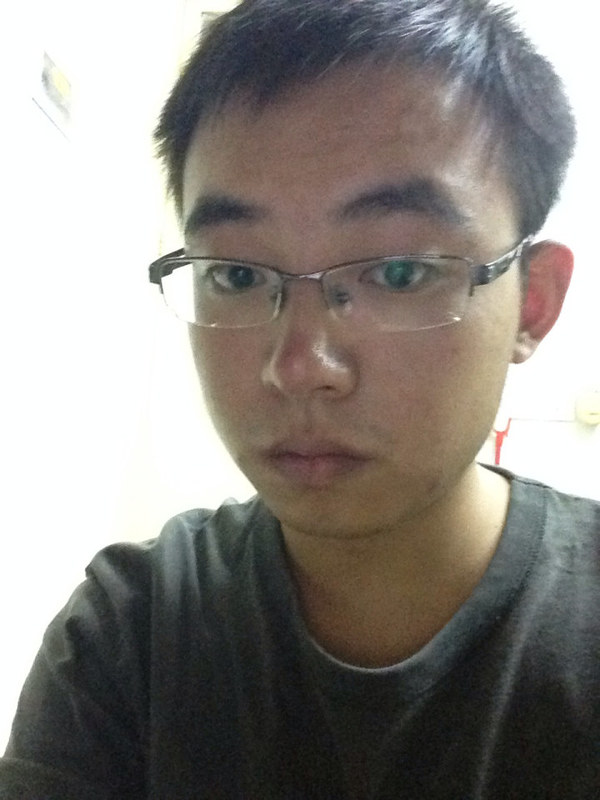
\includegraphics[width=40pt]{photo}
\end{minipage}



\section*{Education}

\begin{itemize}

\item  B.S. in Computer Science.~\quad\qquad~2011.9 - 2015.6~(expected) \\
    \emph{\href{http://acm.sjtu.edu.cn}{ACM Honored Class},
    \href{http://www.sjtu.edu.cn/}{Shanghai Jiao Tong University}.}
\item
    Mianyang High School.\qquad\qquad\quad2008.9 - 2011.6
\end{itemize}

\section*{Personal Experience}
\begin{itemize}
\item \textbf{Research Student}, \emph{\href{http://bcmi.sjtu.edu.cn}{BCMI Lab}}\qquad\qquad\qquad~~2013.7 - present\\
    Advisor:~~~~~~~~~~~~~~{\href{http://bcmi.sjtu.edu.cn/~zhangliqing/}{Prof. Liqing Zhang}}\\
    Research Area:~~~Crowd Density Estimation in videos.
\item \textbf{Teaching Assistant},  \emph{\href{http://acm.sjtu.edu.cn/wiki/Programming_2013}{C++ Programming}}\qquad~ 2013.9 - 2014.1\\
Leader of the TA team.
\item \textbf{Teaching Assistant},  \emph{C++ Programming}\qquad~ 2012.9 - 2013.1\\
Online test maker.
\end{itemize}

\section*{Selected Projects \normalsize{\tt(\href{https://github.com/lostleaf?tab=repositories}{more details})}}
\begin{itemize}
\item \textbf{\href{http://acm.sjtu.edu.cn/ricsrt/}{Ranking Tool Research Capacity in CS}}:
a project for \textbf{\href{http://www.cs.cornell.edu/jeh/}{Prof. John Hopcroft}}'s seminar, which visualizes and compares the CS research productivity, quality and impact of countries and institutions.
\item \textbf{\href{https://github.com/lostleaf/nachos}{Nachos Operating System}}: 
a course project written in Java, including threading and multiprogramming, cache and virtual memory, and a self-designed file system.
\item \textbf{\href{https://github.com/lostleaf/cpu}{Simulated CPU}}:
a course project written in verilog, including a full implementation of tomasulo algorithm with buffers. It is able to execute a turing complete subset of MIPS assembly language.
\item \textbf{\href{https://github.com/lostleaf/compiler}{C Language Compiler}}:
a course project written in Java, which supports most features of C Language and targets the MIPS architecture. It contains a full implementation of several optimization.
\item \textbf{\href{https://github.com/lostleaf/Pathfinding-Evaluation}{Pathfinding Evaluation Framework}}:
a visualized framework written in java for evaluating the performance of pathfinding algorithms working on real-world maps.
\item \textbf{\href{http://acm.sjtu.edu.cn/OnlineJudge/}{SJTU Online Judge}}: (Cooperated with classmates) a publicly available online system written in PHP for testing programs in programming contests, which is used for auto-grading homeworks and exams for several courses and leverages open source softwares such as Linux, nginx, Varnish, MySQL, Redis, memcached, etc.
\end{itemize}

\section*{Awards}
\begin{itemize}
\item  \textbf{First Prize} in China's National Olympiad in Informatics in Provinces (NOIP), 2009. 
\item  \textbf{Silver Medal} in China's National Olympiad in Informatics (NOI), 2010. 
\item  \textbf{Third Prize} in China Undergraduate Mathematical Contest in Modeling (CUMCM), 2013. 
\end{itemize}

\section*{Skills}
\begin{itemize}
\item Basic understanding of Machine Learning and Computer Vision algorithms.
\item Languages and Techniques: Ruby, Java, Python, C/C++, Matlab, javascript, PHP, HTML, Rails, etc.
\end{itemize}

\section*{Personal Statement}
I'm a student in \textbf{\href{http://acm.sjtu.edu.cn}{ACM Honored Class}} of Shanghai Jiaotong University.
I started programming around 2003 and I'm experienced in various programming languages and techniques.
My primary research area is \textbf{machine learning} and \textbf{computer vision}.
My broader interests include {\it web development} and {\it data analysis}.
I would devote myself to the research of Artificial Intelligence.


\end{document}
